\begin{frame}[t] \label{pcuq}
  \frametitle{Polynomial Chaos -- functional representation for RVs}

  \hspace*{4cm}
  \centerline{
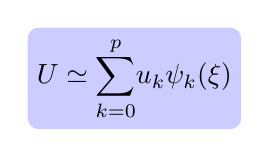
\begin{tikzpicture} \node [rounded corners,fill=blue!20] {
$U\simeq\displaystyle{\sum_{k=0}^{p}} u_k \psi_k(\xi)$
};
\end{tikzpicture}
}

\vspace*{-1.5cm}
  \bi
   \setlength\itemsep{0.2cm}
  \item First introduced by Wiener, 1938
  \item Revitalized by Ghanem and Spanos, 1991
\item Think of Fourier-type expansion
  \item Convergent series if $U$ has finite variance
\item Selection of order $p$ is a modeling choice
\item Describes a r.v. $U$ with a vector of \emph{PC modes} $(u_0, u_1,\dots, u_p)$
\item Utility
\bi
\item Moments: $\EE[u]=u_0$, \ $\mathbb{V}[u]=\sum_{k=1}^K u^2_k ||\Psi_k||^2$, \ $\ldots$
\item Global Sensitivities  -- fractional variances, Sobol' indices
\item Uncertainty propagation
\item Surrogate for forward model
\ei
  \ei


  \mycit{Wiener, 1938;  Ghanem \& Spanos, 1991;  Xiu \& Karniadakis, 2002; Le Ma\^{i}tre \& Knio, 2010}


%  Input parameter domain often dictates the most
%convenient choice of PC
%Polynomials can also be tailored to be orthogonal w.r.t.
%chosen, arbitrary density
\end{frame}

